\documentclass{sig-alternate}

\begin{document}
%
% --- Author Metadata here ---
\conferenceinfo{18-697}{Fall '14 Pittsburgh, PA USA}
\CopyrightYear{2014}
% --- End of Author Metadata ---

\title{Clustering for Controlling Stochastic Optimization using Feedback}
\subtitle{Applied to Newspaper Article Title Category Prediction}

\numberofauthors{2} 
\author{
\alignauthor
Kevin Brennan\\
       \affaddr{Carnegie Mellon University}\\
       \affaddr{5000 Forbes Avenue}\\
       \affaddr{Pittsburgh, PA}\\
       \email{kbrennan@andrew.cmu.edu}
% 2nd. author
\alignauthor
Gavriel Adler\\
       \affaddr{Carnegie Mellon University}\\
       \affaddr{5000 Forbes Avenue}\\
       \affaddr{Pittsburgh, PA}\\
       \email{gya@andrew.cmu.edu}\\
}


\maketitle
\begin{abstract}
Our Abstract
\end{abstract}

%%@Kevin-->Not sure what these are
% A category with the (minimum) three required fields
%\category{H.4}{Information Systems Applications}{Miscellaneous} %I commented out this line
%A category including the fourth, optional field follows...
%\category{D.2.8}{Software Engineering}{Metrics}[complexity measures, performance measures] %I commented out this line

\terms{Classification, Feedback, Stochastic Optimization} %I put some down...

\keywords{Controlled Clustering, Naive Bayes, KMeans, Title Category Classification} %I put some down...

\section{Introduction}
Our Intro

\section{Background}
Background

\section{Method}
\begin{figure*}[t]
\centering
\fbox{
  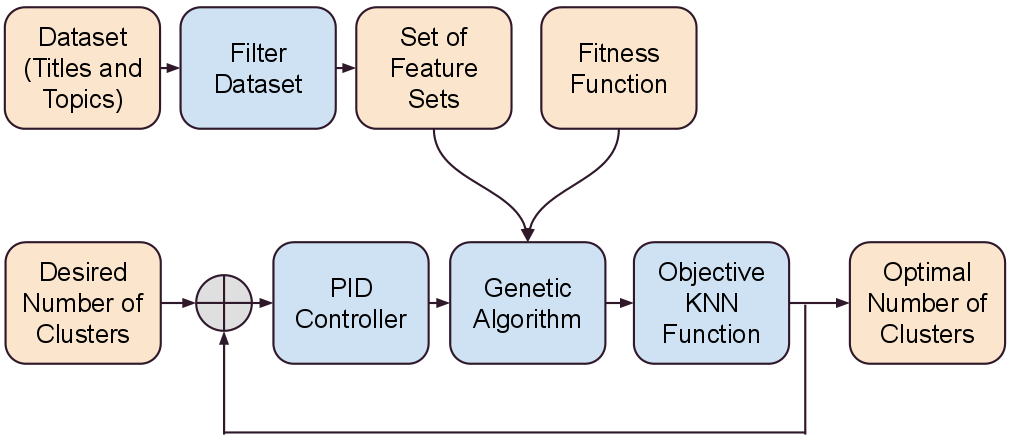
\includegraphics[width=0.8\textwidth]{pipeline.png}}
\caption{The Algorithm Pipeline}
\label{fig:pipeline}
\end{figure*}
\subsection{The Pipeline}
Our pipeline, as seen in Figure~\ref{fig:pipeline}, consists of a few independent pieces put together in a control loop.

\subsection{Genetic Algorithm}
\begin{figure}[t]
\centering
\fbox{\rule{0pt}{2in}
  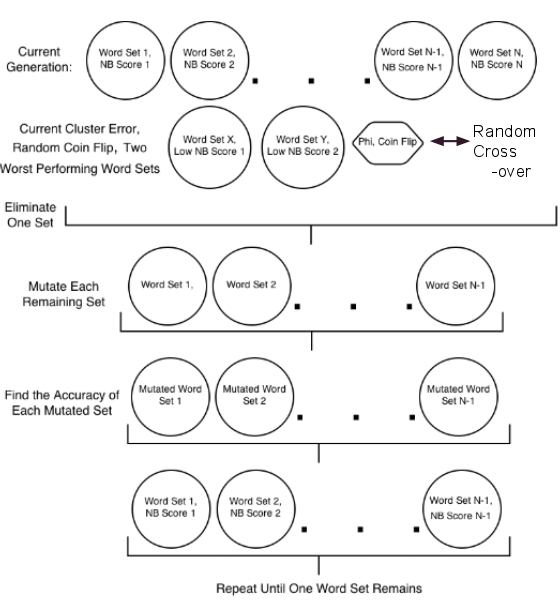
\includegraphics[width=0.5\textwidth]{genetic_algo.png}}
\caption{The flow of one iteration of the genetic algorithm}
\label{fig:genetic_algo}
\end{figure}

\subsection{Clustering Algorithm}

\subsection{Controller}

\section{Results}

\section{Conclusions}

\section{Future Work}

\section{Acknowledgments}

\cite{salas:calculus}

%
% The following two commands are all you need in the
% initial runs of your .tex file to
% produce the bibliography for the citations in your paper.
\bibliographystyle{abbrv}
\bibliography{sigproc}  % sigproc.bib is the name of the Bibliography in this case

\end{document}
